\documentclass[../main.tex]{subfiles}
\graphicspath{{\subfix{../images/}}}
\begin{document}

\subsection{Baseline Multi Layer Perceptron Model}

The Multi Layer Perceptron Model (MLP) is a machine learning model that takes an array of values as an input and passes that it through several layers of processing to get an output. To evaluate its effectiveness, a MLP model was created with a single hidden layer of 150 perceptrons. 

\begin{figure}[h!]
  \centering
  \begin{subfigure}[b]{0.7\linewidth}
    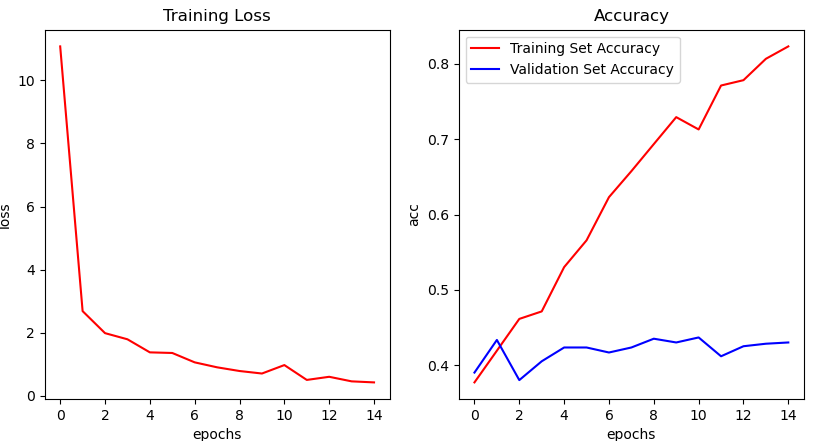
\includegraphics[width=\linewidth]{mlp-performance.png}
  \end{subfigure}
  \caption{Performance of the MLP}
  \label{fig:mlp-validation}
\end{figure}

In the graphs presented the red line represents accuracy of the model on the training set and the blue line represents the accuracy on the validation set. We see that the MLP barely improve on its initial accuracy within 4 epoch. When the train model was used on the test set it achieved an accuracy of 37.89\%. 

\end{document}